%https://tikz.dev/tikz-graphs

%https://gateoverflow.in/166239/ugc-net-cse-november-2017-part-2-question-5

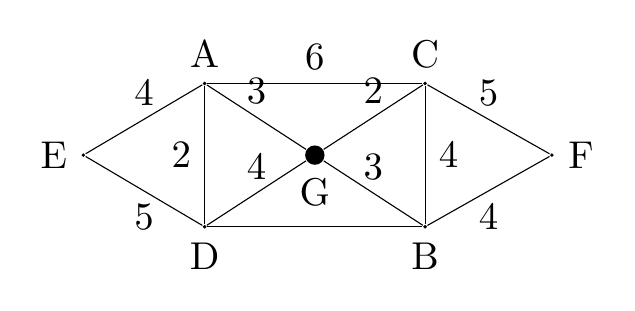
\begin{tikzpicture}[scale = 0.7,transform shape,minimum size=1pt]
\tikzstyle{mynode}=[circle,fill,inner sep=0pt,minimum size=1pt]

\node[mynode] (e) at (0.8,3)[label={left:E}]  {};
\node[mynode] (a) at (3,4.3)[label={above:A}] {};
\node[mynode] (d) at (3,1.7) [label={below:D}]{};
\node[mynode] (c) at (7,4.3)[label={above:C}] {};
\node[mynode] (b) at (7,1.7) [label={below:B}]{};
\node[mynode] (f) at (9.3,3)[label={right:F}] {};
\node[mynode,minimum size=5pt] (g) at (5,3)[label={below:G}] {};

\draw [-] (e) edge node[above] {$4$} (a);
\draw [-] (a) edge node[left] {$2$} (d);
\draw [-] (e) edge node[below] {$5$} (d);
\draw [-] (a) edge node[above] {$6$} (c);

\draw [-] (a) edge node[above] {$3$} (g);
\draw [-] (d) edge node[above] {$4$} (g);
\draw [-] (g) edge node[above] {$3$} (b);
\draw [-] (d) edge node[above] {} (b);

\draw [-] (c) edge node[above] {$5$} (f);
\draw [-] (b) edge node[below] {$4$} (f);
\draw [-] (c) edge node[right] {$4$} (b);
\draw [-] (c) edge node[above] {$2$} (g);


\end{tikzpicture}




%https://gateoverflow.in/333236/gate-cse-2020-question-ga-5
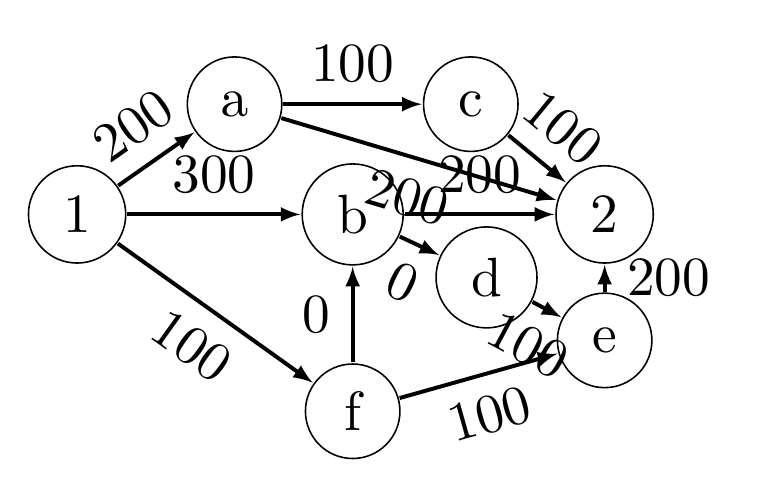
\begin{tikzpicture}[>=latex,shorten >=0.1pt,auto, thick,node distance=2.0cm]
\node (a) [draw , circle, minimum size= 0.5cm, line width=0.2mm] at (0.0,0.3) {1};
\node (b) [draw , circle, minimum size= 0.6cm, line width=0.2mm] at (2.0,1.7) {a};
\node (c) [draw , circle, minimum size= 0.6cm, line width=0.2mm] at (5.0,1.7) {c};
\node (d) [draw , circle, minimum size= 0.5cm, line width=0.2mm] at (3.5,0.3) {b};
\node (e) [draw , circle, minimum size= 0.5cm, line width=0.2mm] at (6.7,0.3) {2};
\node (f) [draw , circle, minimum size= 0.6cm, line width=0.2mm] at (3.5,-2.2) {f};
\node (g) [draw , circle, minimum size= 0.6cm, line width=0.2mm] at (6.7,-1.3) {e};
\node (h) [draw , circle, minimum size= 0.5cm, line width=0.2mm] at (5.2,-0.5) {d};
\path[->,line width=0.5mm]
(a) edge              node [sloped,above] {200} (b)
(b) edge              node {100} (c)
(c) edge              node [above,sloped] {100} (e)
(b) edge              node [below,sloped] {200} (e)
(a) edge              node {300} (d)
(d) edge              node {200} (e)
(d) edge              node [below ,sloped] {0} (h)
(h) edge              node [below,sloped] {100} (g)
(g) edge              node [right]{200} (e)
(a) edge              node [below, sloped] {100} (f)
(f) edge              node [below,sloped] {100} (g)
(f) edge              node [left] {0} (d);
\end{tikzpicture}



%https://gateoverflow.in/204122/gate2018-47
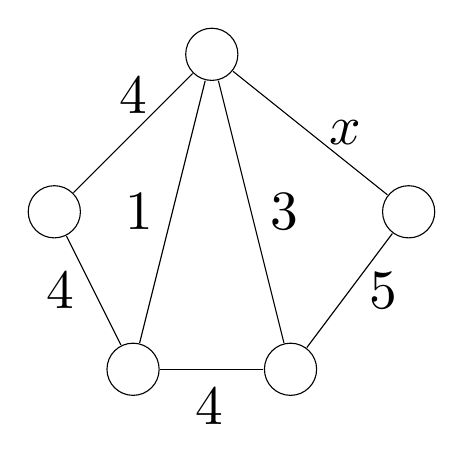
\begin{tikzpicture}
\tikzstyle{every node}=[scale=2,auto]

\node[shape=circle,draw=black] (A) at (-2,0) {};
\node[shape=circle,draw=black] (B) at (0,2) {};
\node[shape=circle,draw=black] (C) at (2.5,0) {};
\node[shape=circle,draw=black] (D) at (-1,-2) {};
\node[shape=circle,draw=black] (E) at (1,-2) {};
   
\path [-] (A) edge node[above] {$4$} (B);
\path [-] (B) edge node[right] {$x$} (C);
\path [-] (C) edge node[right] {$5$} (E);
\path [-] (E) edge node[right] {$3$} (B);
\path [-] (E) edge node[below left,pos = 0.2] {$4$} (D);
\path [-] (D) edge node[left] {$4$} (A);
\path [-] (D) edge node[left] {$1$} (B);
   
\end{tikzpicture}









